\documentclass[11pt,letterpaper]{article}

\usepackage[utf8]{inputenc}
\usepackage[spanish,es-nodecimaldot]{babel}
\usepackage{graphicx}
\usepackage{spverbatim}
\usepackage{amsmath}
\usepackage{amssymb}

\usepackage[top=1in, bottom=1in, left=1in, right=1in]{geometry}

\begin{document}

\begin{titlepage}
    \centering

    {\scshape\LARGE Universidad Nacional Autónoma de México \par}

    \vspace{1cm}
    {\scshape\Large Facultad de Ciencias\par}
    \vspace{1.5cm}

    \begin{center}
        
\includegraphics[scale=.1]{../../assets/img/logo.png}
    \end{center}

    \vspace{.8 cm}

    {\LARGE Práctica 01: \par}
    {\huge\bfseries Compilador \par}

    \vspace{0.5cm}
    {\large\itshape Pablo A. Trinidad Paz\par}

    \vfill

    Trabajo presentado como parte del curso de \textbf{Introducción a Ciencias de la Computación}
    impartido por la profesora \textbf{Verónica Esther Arriola Ríos}. \par
    \vspace{0.1cm}
    {\large 24 de agosto de 2018\par}
\end{titlepage}

{\Large \bfseries Los programas de la JDK \par}

\begin{enumerate}
    \item [Actividad 1.2] {\bfseries Escribe exactamente que archivos fueron creados y donde:\par}

        Dentro de \texttt{Reloj/src/icc/practica1} los siguientes archivos fueron creados:
        \begin{enumerate}
            \item [1.] \texttt{ClaseReloj.class}
            \item [2.] \texttt{PanelDeReloj.class}
            \item [3.] \texttt{Reloj.class}
            \item [4.] \texttt{TiempoSistema.class}
            \item [5.] \texttt{UsoReloj.class}
            \item [6.] \texttt{VistaReloj.class}
            \item [7.] \texttt{VistaRelojAnalogico.class}
            \item [8.] \texttt{VistaRelojAnalogico\$1.class}
        \end{enumerate}

    \item [Actividad 1.3] {\bfseries Ejecuta \texttt{UsoReloj}\par}
            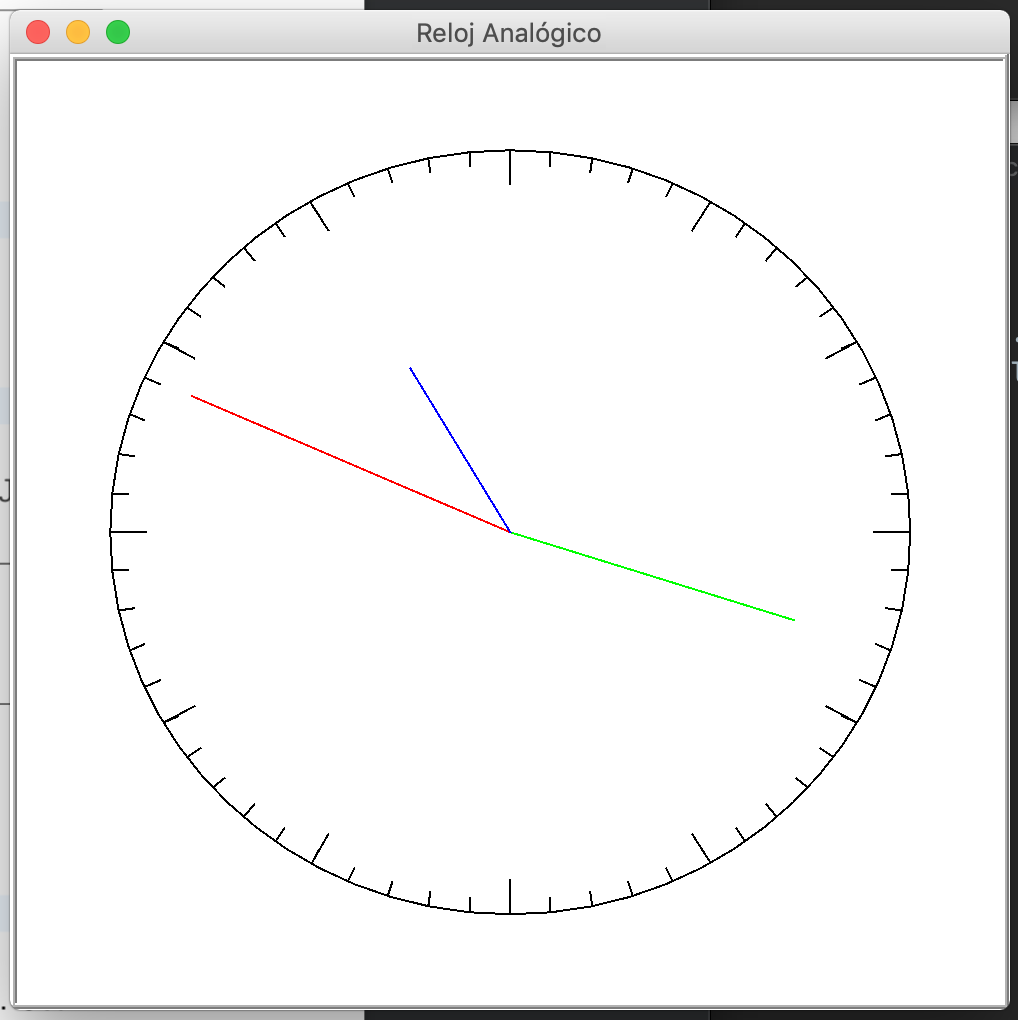
\includegraphics[scale=.3]{assets/img/1-3.png}

    \item [Actividad 1.4] {\bfseries Intenta invocar a la máquina virtual con los
    nombres de otros archivos \texttt{.class}. ¿Qué sucede? Lee lo que devuelve la consola
    y abre los archivos \texttt{.java} correspondientes que necesites. ¿Qué tiene el archivo
    \texttt{UsoReloj.java} que permite invocar su \texttt{.class} con java? \par}

        Al tratar de ejecutar otros archivos diferentes a \texttt{UsoReloj.class}, Java
        busca un método principal, \texttt{Main method}, que le especifique qué operaciones
        tiene que ejecutar para iniciar. Lo que tiene diferente el archivo
        \texttt{UsdoReloj.java} que permite que la ejecución de la aplicación suceda es la
        implementación del método \texttt{main} en la línea $16$, que además está definido
        como público, estático y que no regresa ningún valor al terminar la ejecución.

    \vfill

    \item [Actividad 1.6] {\bfseries Generar la documentación de \texttt{practica1}. ¿Qué observas? \par}

        Se genearon archivos para servir un sitio web estático como: HTMLs, CSSs y archivos de
        \mbox{JavaScript}. Al acceder al website de los documentos podemos ver el listado de clases,
        descripción de cada una de ellas y dentro de cada una sus métodos, atributos, etc.

        El website luce así:

        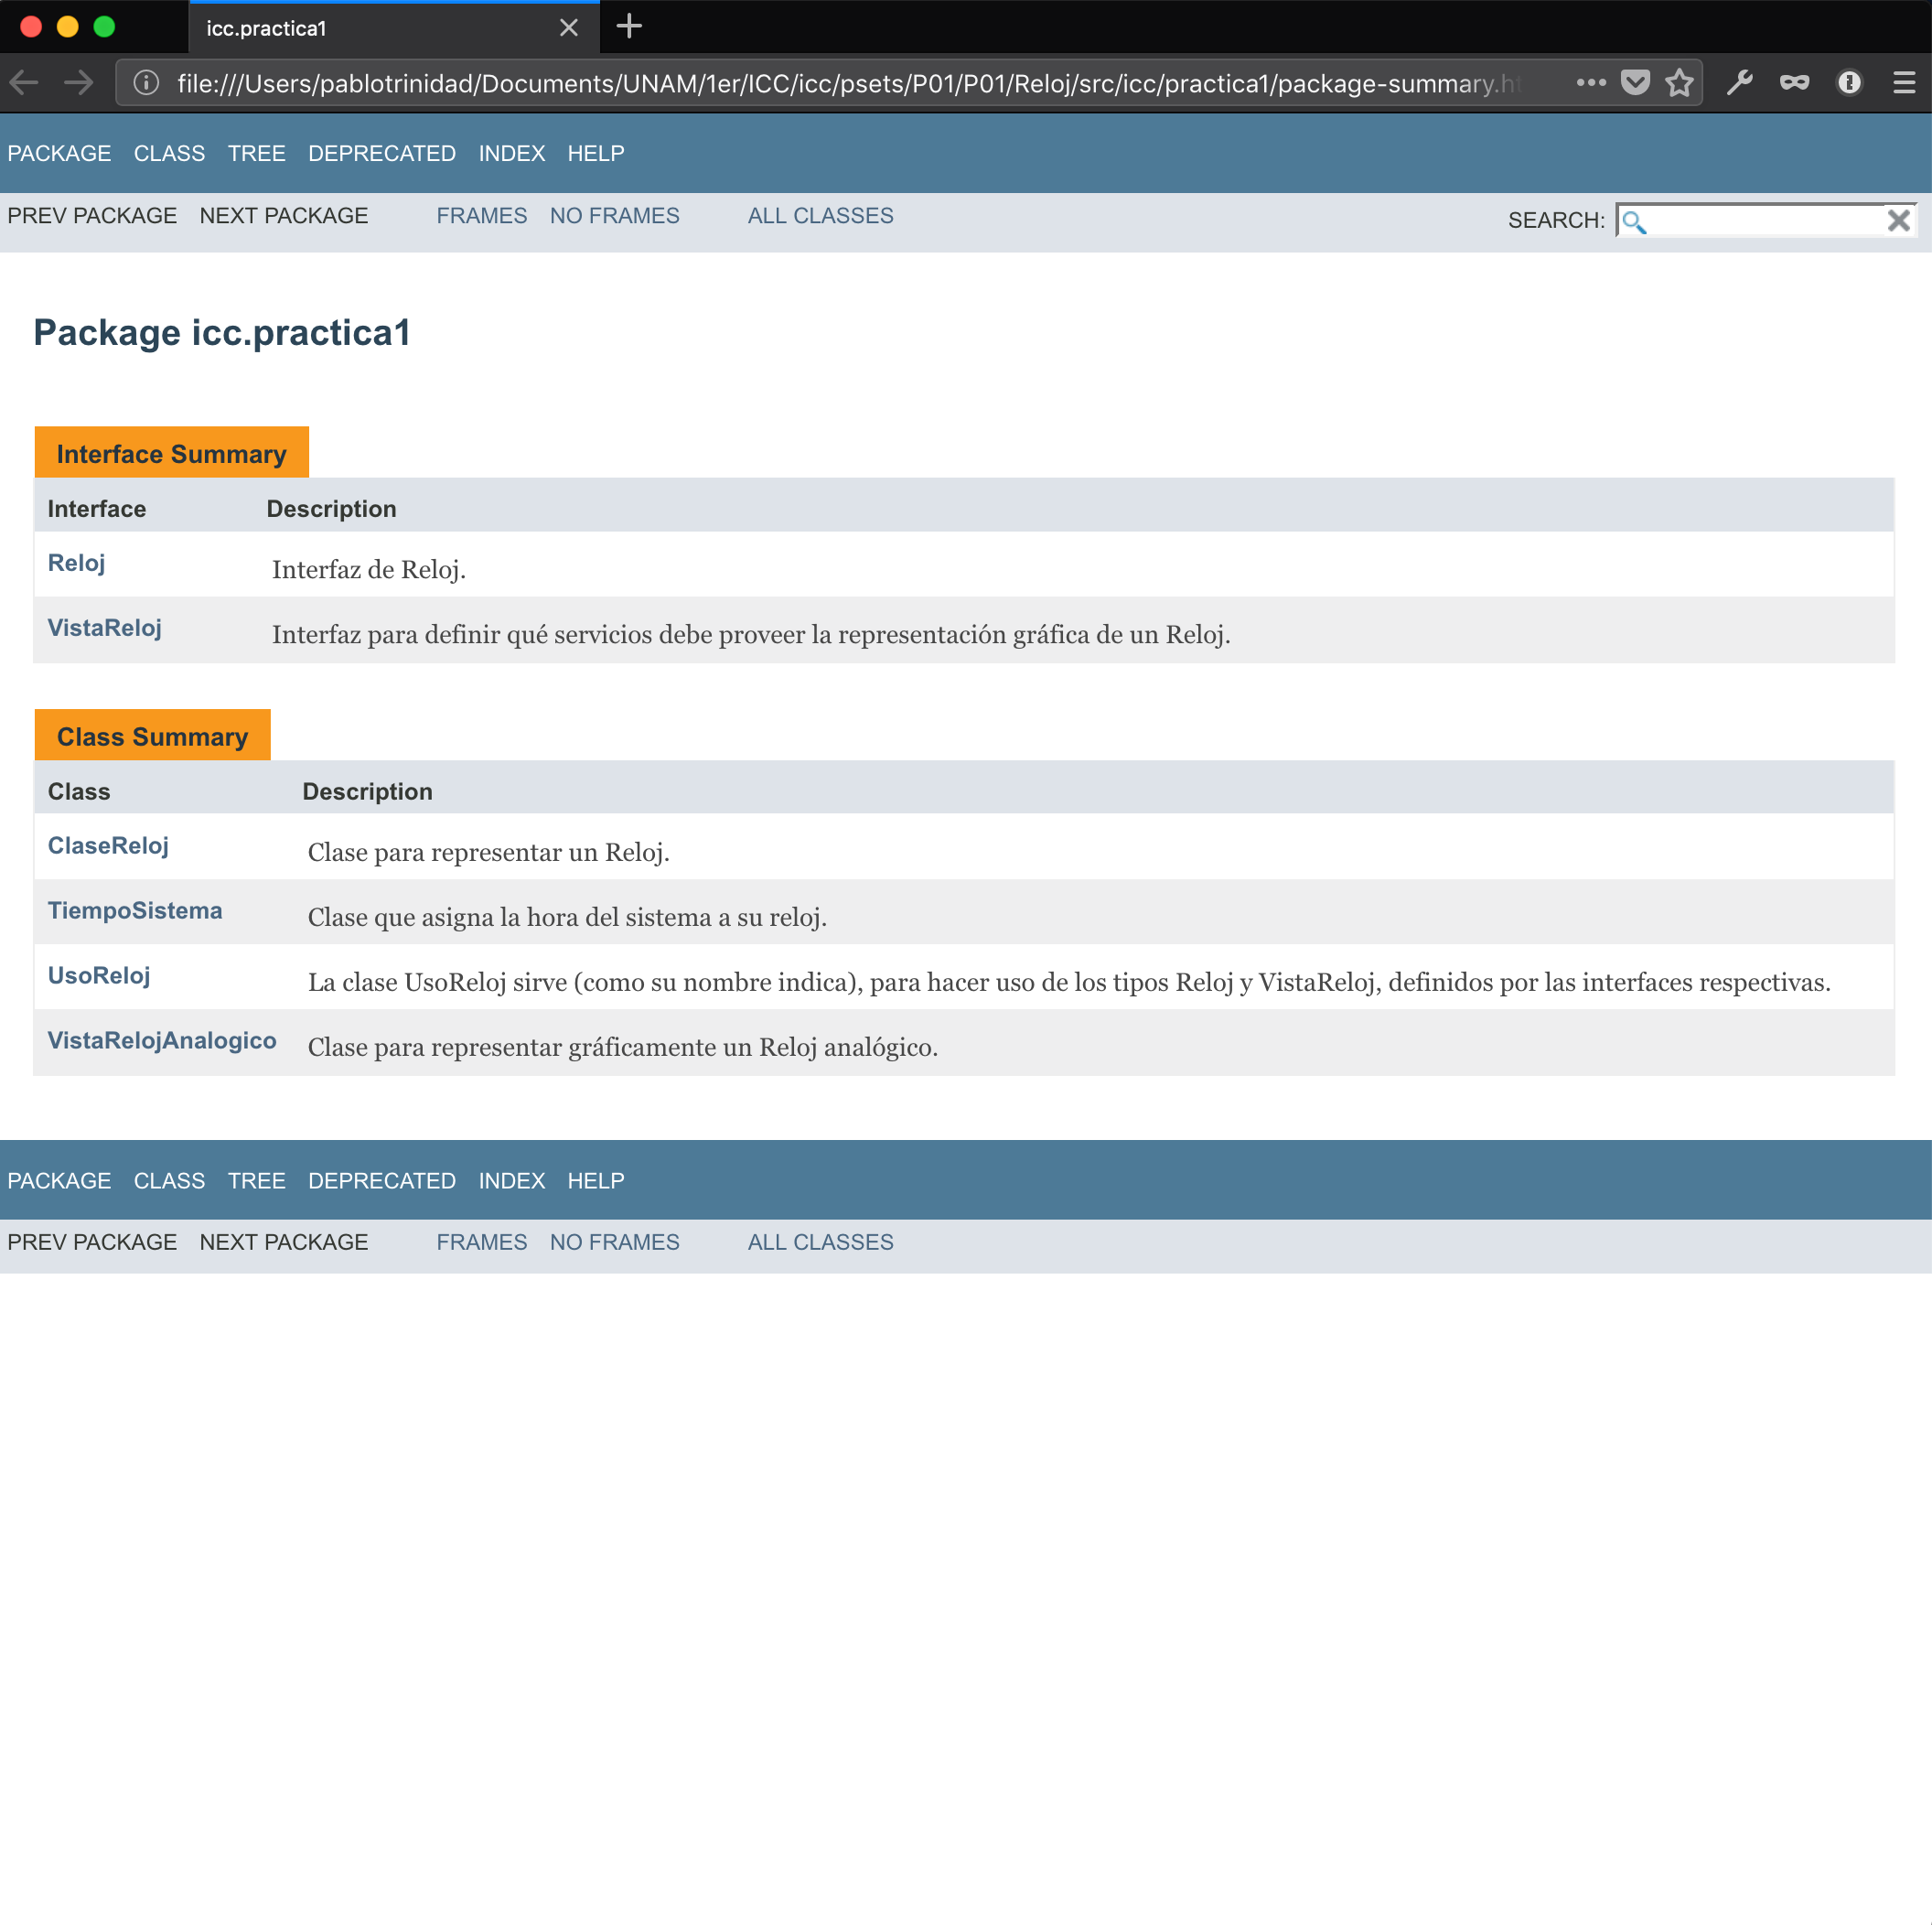
\includegraphics[scale=.3]{assets/img/1-6.png}

\end{enumerate}

{\Large \bfseries Usando una herammienta auxiliar: ant \par}

Las siguientes respuestas corresponden a las actividades, ejercicios y preguntas
de la \textbf{Práctica 1} del Manual de Prácticas de Introducción a las Ciencias
de la Computación escrito por \textbf{Canek Peláez V.} y \textbf{Elisa Viso G.}.

\begin{enumerate}
    \item [Actividad 1.1] {\bfseries Al invocar el comando \texttt{javac} Anota todas las opciones que se pueden pasar al compilador. \par}
        \begin{itemize}
            \item \texttt{@<filename>}: Read options and filenames from file
            \item \texttt{-Akey[=value]}: Options to pass to annotation processors
            \item \texttt{--add-modules <module>(,<module>)*}: Root modules to resolve in addition to the initial modules, or all modules on the module path if <module> is ALL-MODULE-PATH.
            \item \texttt{--boot-class-path <path>, -bootclasspath <path>}: Override location of bootstrap class files
            \item \texttt{--class-path <path>, -classpath <path>, -cp <path>}: Specify where to find user class files and annotation processors
            \item \texttt{-d <directory>}: Specify where to place generated class files
            \item \texttt{-deprecation}: Output source locations where deprecated APIs are used
            \item \texttt{-encoding <encoding>}: Specify character encoding used by source files
            \item \texttt{-endorseddirs <dirs>}: Override location of endorsed standards path
            \item \texttt{-extdirs <dirs>}: Override location of installed extensions
            \item \texttt{-g}: Generate all debugging info
            \item \texttt{-g: lines,vars,source}: Generate only some debugging info
            \item \texttt{-g}:none: Generate no debugging info
            \item \texttt{-h <directory>}: Specify where to place generated native header files
            \item \texttt{--help, -help}: Print this help message
            \item \texttt{--help-extra, -X}: Print help on extra options
            \texttt{-implicit: none,class}: Specify whether or not to generate class files for implicitly referenced \item files
            \item \texttt{-J<flag>}: Pass <flag> directly to the runtime system
            \item \texttt{--limit-modules <module>(,<module>)*}: Limit the universe of observable modules
            \item \texttt{--module <module-name>, -m <module-name>}: Compile only the specified module, check timestamps
            \item \texttt{--module-path <path>, -p <path>}: Specify where to find application modules
            \texttt{--module-source-path <module-source-path>}: Specify where to find input source files for multiple \item modules
            \item \texttt{--module-version <version>}: Specify version of modules that are being compiled
            \item \texttt{-nowarn}: Generate no warnings
            \item \texttt{-parameters}: Generate metadata for reflection on method parameters
            \item \texttt{-proc: none,only}: Control whether annotation processing and/or compilation is done.
            \texttt{-processor <class1>[,<class2>,<class3>...]}: Names of the annotation processors to run; bypasses \item default discovery process
            \item \texttt{--processor-module-path <path>}: Specify a module path where to find annotation processors
            \item \texttt{--processor-path <path>, -processorpath <path>}: Specify where to find annotation processors
            \item \texttt{-profile <profile>}: Check that API used is available in the specified profile
            \item \texttt{--release <release>}: Compile for a specific VM version. Supported targets: 10, 6, 7, 8, 9
            \item \texttt{-s <directory>}: Specify where to place generated source files
            \item \texttt{-source <release>}: Provide source compatibility with specified release
            \item \texttt{--source-path <path>, -sourcepath <path>}: Specify where to find input source files
            \item \texttt{--system <jdk>|none}: Override location of system modules
            \item \texttt{-target <release>}: Generate class files for specific VM version
            \item \texttt{--upgrade-module-path <path>}: Override location of upgradeable modules
            \item \texttt{-verbose}: Output messages about what the compiler is doing
            \item \texttt{--version, -version}: Version information
            \item \texttt{-Werror}: Terminate compilation if warnings occur
        \end{itemize}

    \item [Ejercicio 3] {\bfseries Ejecutar \texttt{ant clean} y
        \texttt{touch src/icc/practica1/UsoReloj.java} y explicar la diferencia
        de correr \texttt{ant} antes y después de haber sobreescrito \texttt{UsoReloj.java}\par}

        Durante la primera ejecución de \texttt{ant}, la salida del programa decía que
        estaba compilando 6 archivos fuente mientras que en la segunda ejecución de
        \texttt{ant} la salida decía que únicamente estaba compilando un archivo:

        \begin{center}
            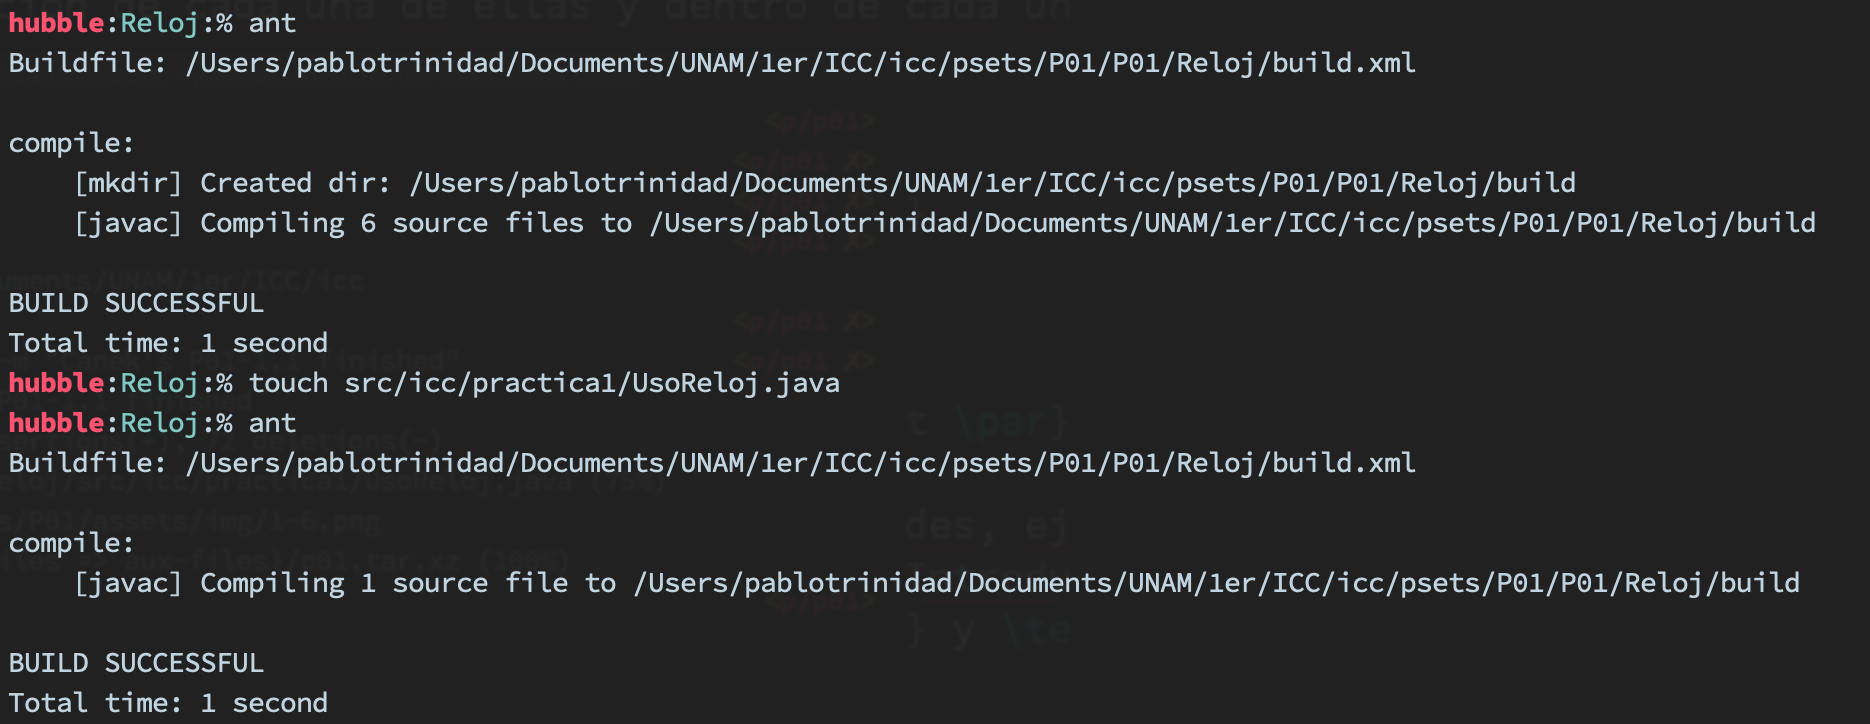
\includegraphics[scale=.5]{assets/img/canek-e-3.png}
        \end{center}

        Este comportamiento se debe a que el archivo \texttt{UsoReloj.java} es
        el archivo principal que desencadena la ejecución completa de la aplicación
        y logra esto haciendo uso de los otros 5 archivos restantes.

        Al momento en que nosotros usamos \texttt{touch UsoReloj.java}, el contenido
        del archivo \texttt{UsoReloj.java} es borrado y queda un archivo vacío. Después,
        cuando ejecutamos \texttt{ant}, o en su defecto \texttt{javac}, estos inician
        el proceso de compilación en un sólo archivo (al igual que en el caso previo) pero
        con la diferencia de que este nuevo, y vacío, archivo nunca hace referencia a
        los otros 5.

    \item [Pregunta 1] {\bfseries ¿Qué errores encontraste al compilar
    esta práctica? Explica en qué consisten.\par}

        \begin{itemize}
            \item \texttt{not a statement}: Que hacía referencia a que una construcción
                del tipo \texttt{objeto.metodo)} no es correcta y debía ser cambiada por
                algo del tipo \texttt{objeto.metodo()}.

            \item \texttt{error: 'symbol' expected}: Donde \texttt{symbol} podría ser
            un \texttt{;}, \texttt{)}, \texttt{(} o cualquier elemtento de la sintaxis
            de Java que fuera requerido en la expresión formada pero que resultaba faltante
            o se encontraba sustituido por uno incorrecto.

            \item \texttt{cannot find symbol}: Que significaba que se estaba haciendo
            uso de una variable que no había sido definida anteriormente. En el ejemplo
            de la práctica, el error estaba en haber escrito \texttt{relog} en lugar de
            \texttt{reloj}.

            \item \texttt{method X cannot be applied to given types}: Que significaba que
            un método de una clase estaba esperando recibir ciertos parámetros de cierto
            tipo y recibió otros diferentes a los especificados. En el ejemplo de la
            práctica, el error estaba cuando se llamaba el método \texttt{espera} desde una
            instancia de la clase \texttt{VistaRelojAnalogico} sin pasarle el entero positivo
            que el método estaba esperando.
        \end{itemize}

    \item [Pregunta 2] {\bfseries Los errores que encontraste, ¿de qué tipo crees que sean,
    sintácticos o semánticos? Justifica tu respuesta. \par}

        Ambos. Sintácticos porque en algunos casos hacían falta símbolos para delimitar
        el fin de una sentencia (\texttt{;}) o la llamada a un método (\texttt{()}) pero
        de la misma manera había errores semánticos, es decir, relacionados al significado
        del contenido escrito. Por ejemplo: Llamar a la variable inexistente \texttt{relog}
        o ejecutar el método \texttt{espera} de la clase \texttt{VistaRelojAnalogico} sin
        mandarle los argumentos necesarios para que se ejecutara.

    \item [Pregunta 3] {\bfseries ¿Cuántos archivos en bytecode (los que tienen extensión
    \texttt{.class}) se generaron?\par}

        8 archivos \texttt{.class}

        \begin{center}
            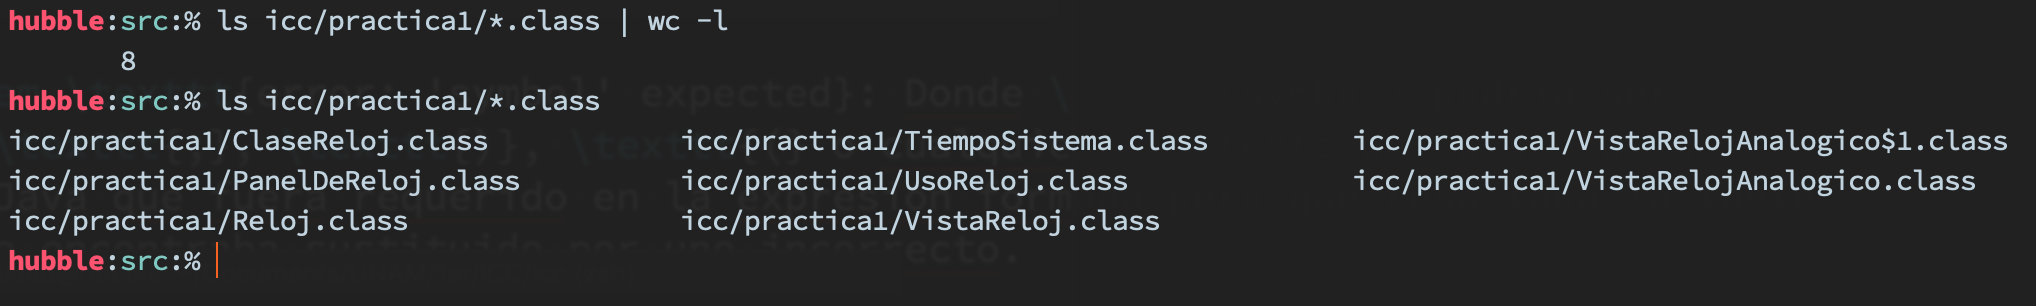
\includegraphics[scale=.4]{assets/img/canek-p-3.png}
        \end{center}

    \item [Pregunta 4] {\bfseries ¿Cuál crees que sea la explicación del comportamiento de
    Ant después de hacer el ejercicio 3? Justifica tu respuesta.\par}

        Como mencioné en la respuesta al \textbf{Ejercicio 3}, se debe a que el archivo
        principal del cual parte la compiliación es diferente antes y después de hacer
        el \texttt{touch}. Antes, el archivo hace uso de los otros 5 mientras que después,
        el archivo está vacío y no usa ninguna otra clase.
\end{enumerate}

{\Large \bfseries Estructura de un programa \par}

\begin{enumerate}
    \item [Actividad 1.7] {\bfseries Ejecuta el programa \texttt{Entrada}
    ¿Qué aparece? Ahora, ejecutalo enviando argumentos ¿Qué obtienes?\par}

        En la primera ejecución el programa regresa el mensaje
        "\texttt{No se recibieron indicaciones.}" y en la segunda ejecución
        el programa regresó la lista de argumentos enviados precedidos por el
        mensaje "\texttt{Argumento $n$:}" donde $n$ será el número del argumento $-1$

    \item [Actividad 1.8] {\bfseries Experimenta con el archivo \texttt{Entrada.jav} y
    reporta lo que hace el programa.\par}

        Ejecutar \texttt{java -jar arg1 arg2 arg3} generará errores ya que el primer
        argumento después de \texttt{-jar} debe la ubicación del \texttt{jarfile}.

        Agregando el argumento \texttt{Entrada.jar} entre \texttt{-jar} y el listado
        de argumentos \texttt{arg1 arg2 arg3} el comando se ejecuta de manera correct
        y podemos observar el mismo comportamiento de listado de argumentos que se
        describe en la \textbf{Actividad 1.7}.

        \begin{center}
            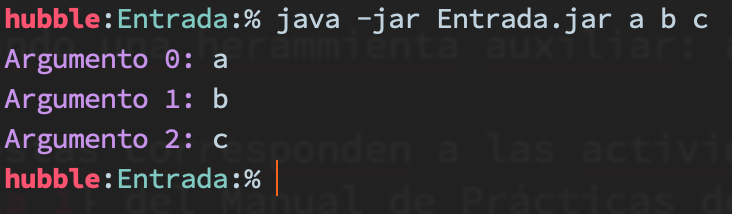
\includegraphics[scale=.5]{assets/img/1-8.png}
        \end{center}

    \item [Actividad 1.10] {\bfseries Lee los dos archivos \texttt{build.xml}
    utilizados en esta práctica y observa en qué se parecen y en qué difieren.
    ¿Qué objetivos reconoce cada archivo? ¿Qué pasos ejecutará cada uno de los
    objetivos (observa el atributo llamado \texttt{depends})?\par}

        Se parecen en que ambos tienen la misma estructura de tags.
        Por ejemplo, ambos comparten las etiquetas \texttt{xml} y \texttt{project}.
        Además, ambos tienen \texttt{targets} definidos que permiten compilar,
        correr, limpiar y generar la documentación del proyecto.

        Difieren en que el \texttt{XML} del programa \texttt{Entrada} define
        más propiedades usando el tag \texttt{propery} mientras que la clase del
        reloj no lo hace. También, se define un \texttt{target} adicional en
        \texttt{Entrada} para distribuir el paquete. Existen más comentarios para
        el \texttt{XML} de \texttt{Entrada} y de la misma manera la tarea default
        está definida como la sucesión de \texttt{clean, build y dist}.

        Cada XML apunta a su resprectivo proyecto y cada target "\texttt{paso}"
        difiere ligeramente de otro.

        Acerca de los \texttt{depends}, especifican que \texttt{target} tiene
        que ser ejecutado antes de que ese puede correr. Por ejemplo, \texttt{run}
        requiere que \texttt{compile} suceda antes.

\end{enumerate}

\end{document}
